\section{Experiment 2 : HTTP}
\subsection{HTTP : The Basic HTTP GET/response interaction}
    \subsubsection*{Problems}
    \begin{enumerate}[label=\bfseries Problem \arabic*:,leftmargin=*,labelindent=1em]
        \item Is your browser running HTTP version 1.0 or 1.1? What version of HTTP is the server running?\\[0.2mm]
            \soln My browser's HTTP version : 1.1 / The server's HTTP version : 1.1
            \vspace{-2mm}  
            \begin{figure}[!h]\centering
        		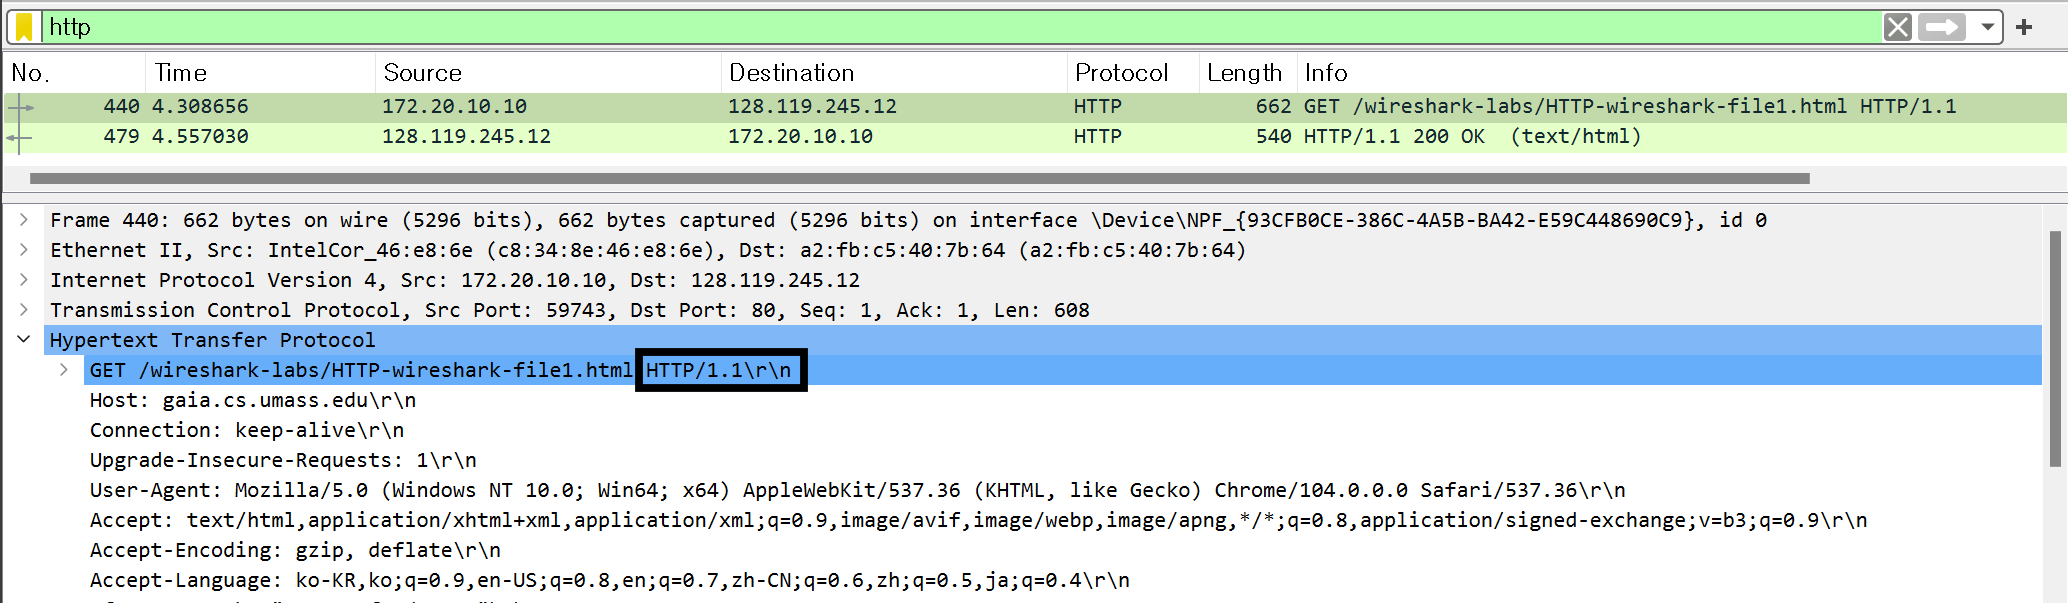
\includegraphics[width=.78\textwidth]{image/result_week01/Q2-1-1.png}
        		\caption{\footnotesize Problem 2-1-1's screenshot : Packet-GET / wireshark-file1.html HTTP/1.1}
        		\vspace{-10pt}
            \end{figure}
            % \vspace{-4mm}  
            \begin{figure}[!h]\centering
        		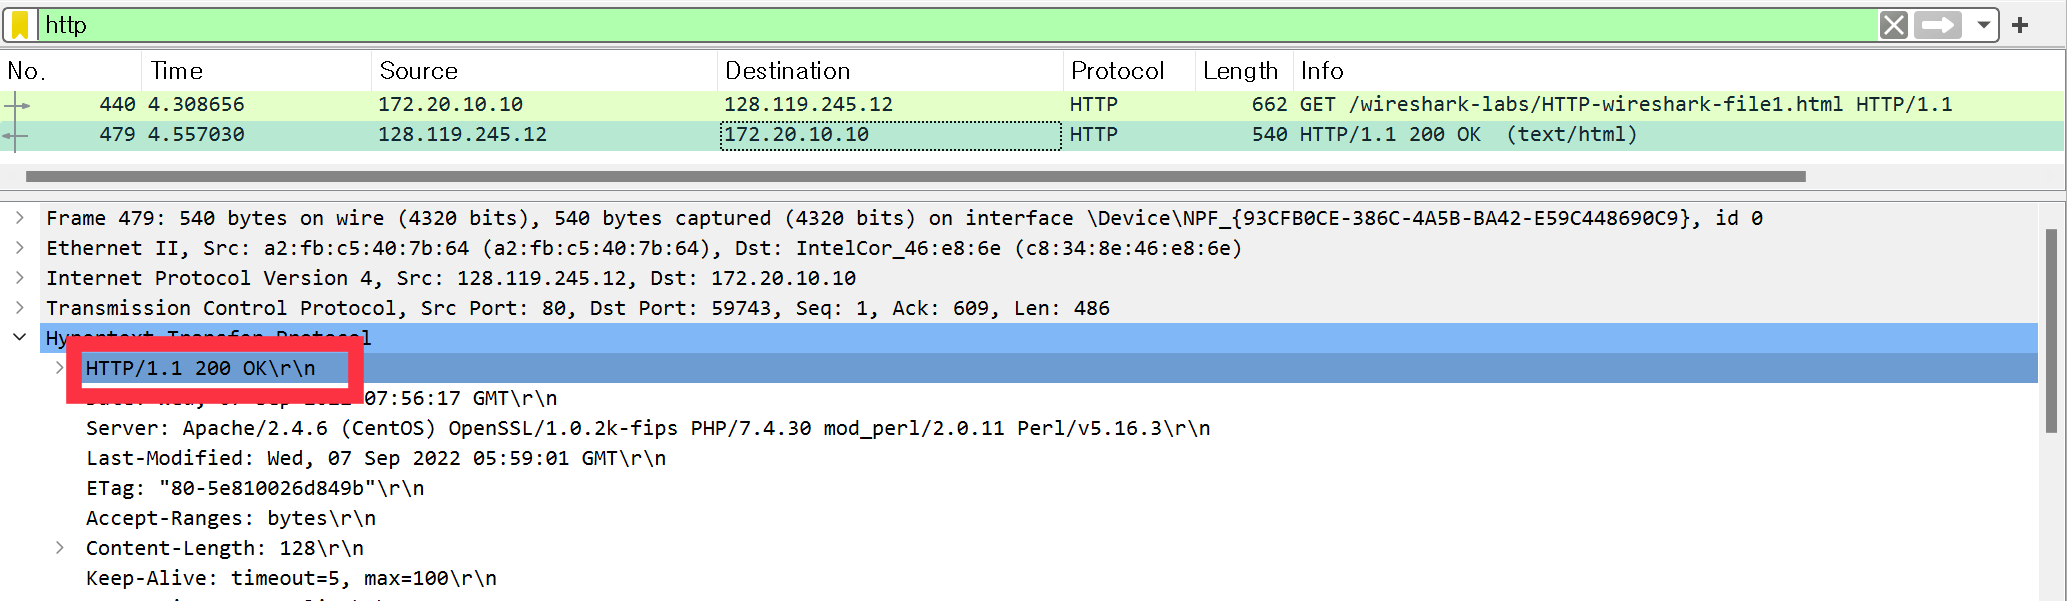
\includegraphics[width=.79\textwidth]{image/result_week01/Q2-1-2.png}
        		\caption{\footnotesize Problem 2-1-2's screenshot : Packet-HTTP/1.1 200 OK}
        		\vspace{-10pt}
            \end{figure}
            
            
            
        \item What languages (if any) does your browser indicate that it can accept to the server?\\[0.2mm]
            \soln Accept-Language : ko-kr
            \vspace{-2mm}  
            \begin{figure}[!h]\centering
        		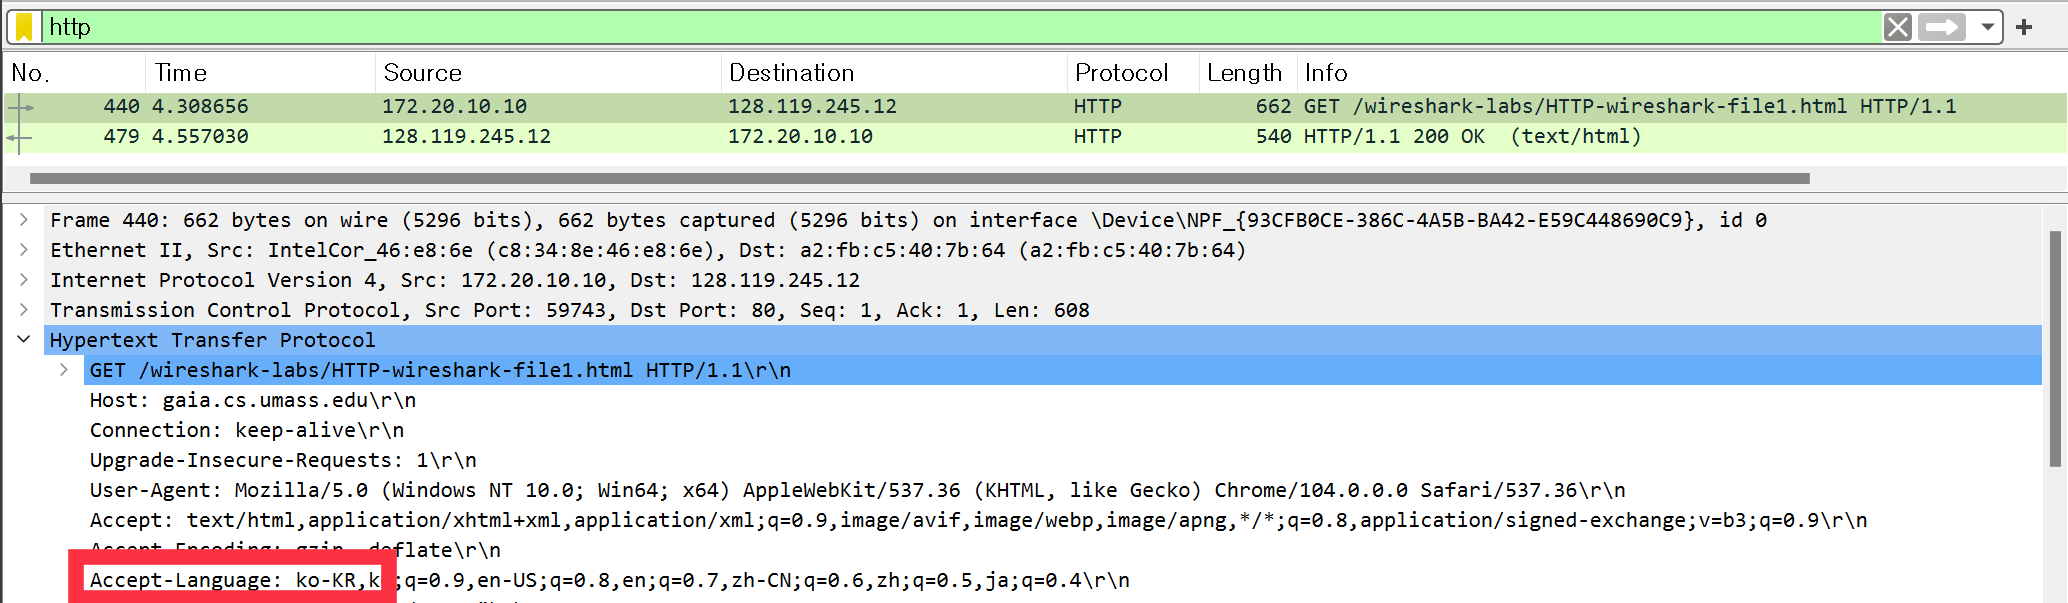
\includegraphics[width=.78\textwidth]{image/result_week01/Q2-2.png}
        		\caption{\footnotesize Problem 2-2's screenshot : Packet-GET / wireshark-file1.html HTTP/1.1}
        		\vspace{-10pt}
            \end{figure}
            % \vspace{-4mm}             
        \item What is the IP address of your computer? Of the gaia.cs.umass.edu server? \\[0.2mm]
            \soln My computer : 172.20.10.10 / gaia.cd.umass.edu : 128.119.245.12
            \vspace{-2mm}  
            \begin{figure}[!h]\centering
        		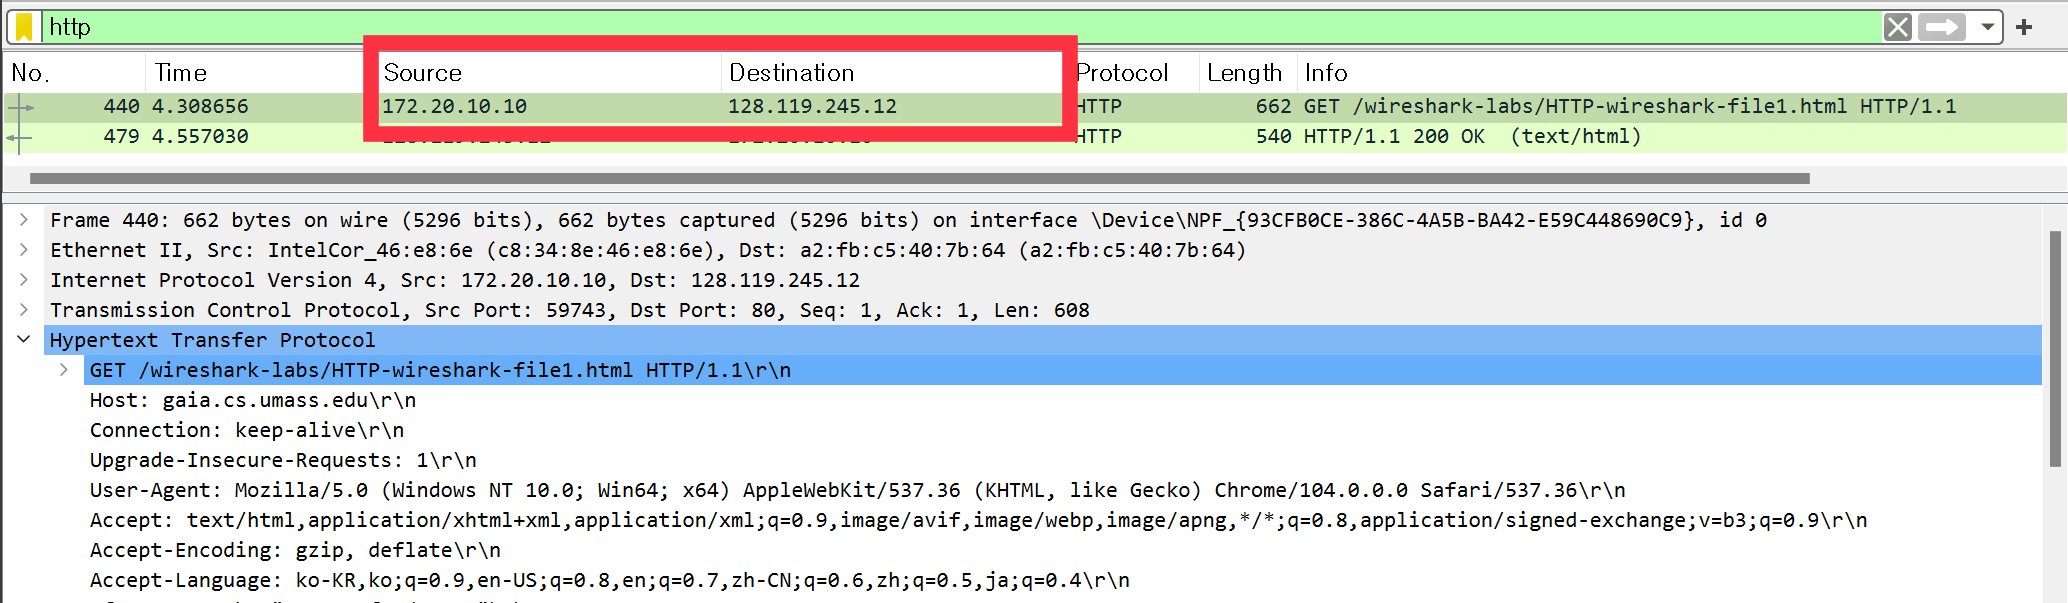
\includegraphics[width=.78\textwidth]{image/result_week01/Q2-3.png}
        		\caption{\footnotesize Problem 2-3's screenshot : Packet-GET / wireshark-file1.html HTTP/1.1}
        		\vspace{-10pt}
            \end{figure}
            % \vspace{-4mm}      
\newpage
        \item What is the status code returned from the server to your browser?\\[0.2mm]
            \soln status code : 200 OK
            \vspace{-2mm}  
            \begin{figure}[!h]\centering
        		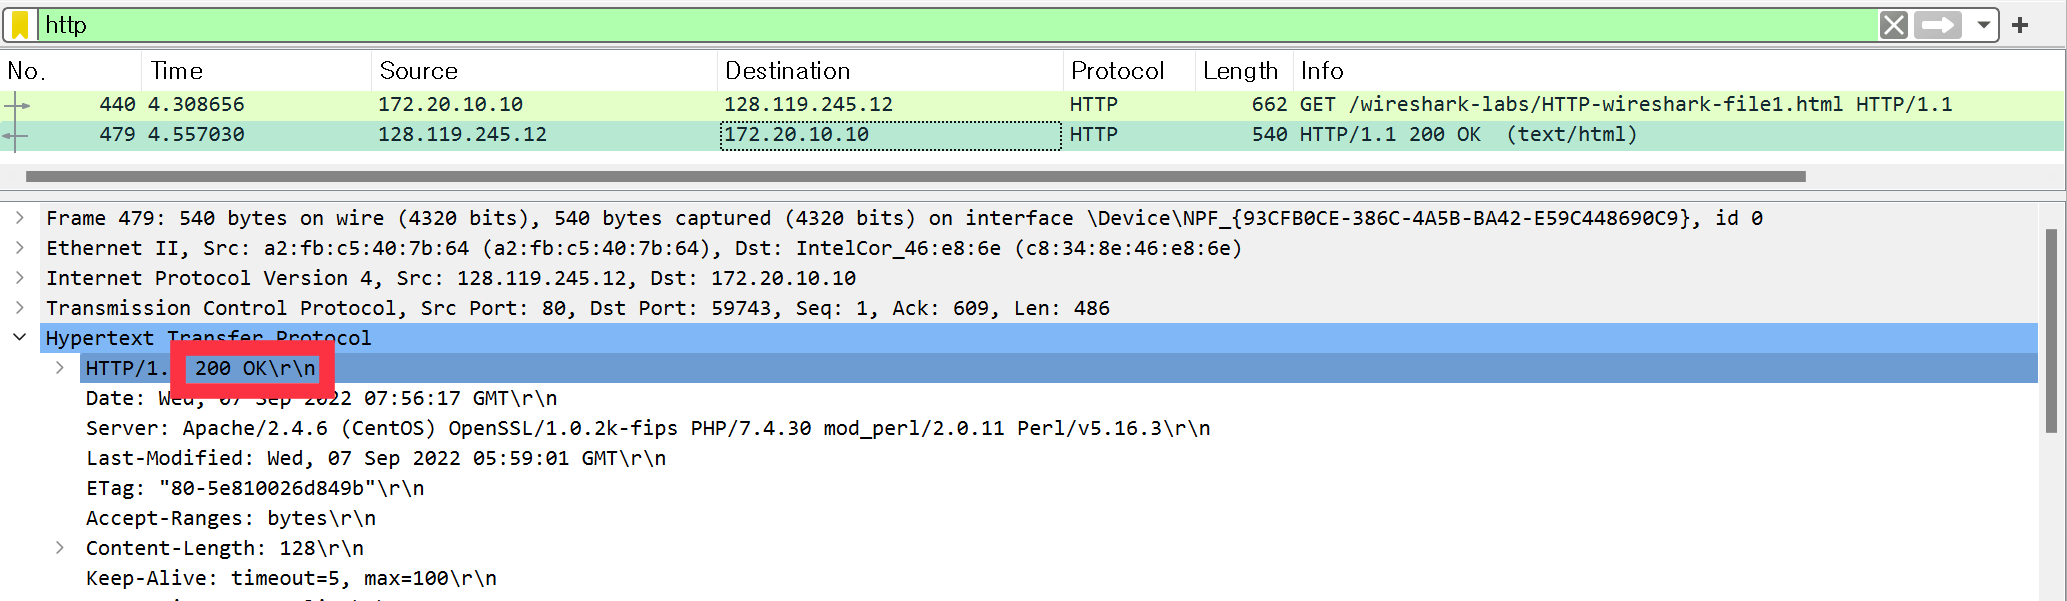
\includegraphics[width=.79\textwidth]{image/result_week01/Q2-4.png}
        		\caption{\footnotesize Problem 2-4's screenshot : Packet-HTTP/1.1 200 OK}
        		\vspace{-10pt}
            \end{figure}            
        \item When was the HTML file that you are retrieving last modified at the server? \\[0.2mm]
            \soln Last-Modified : Wed, 07 Sep 2022 05:59:01 GMT
            \vspace{-2mm}  
            \begin{figure}[!h]\centering
        		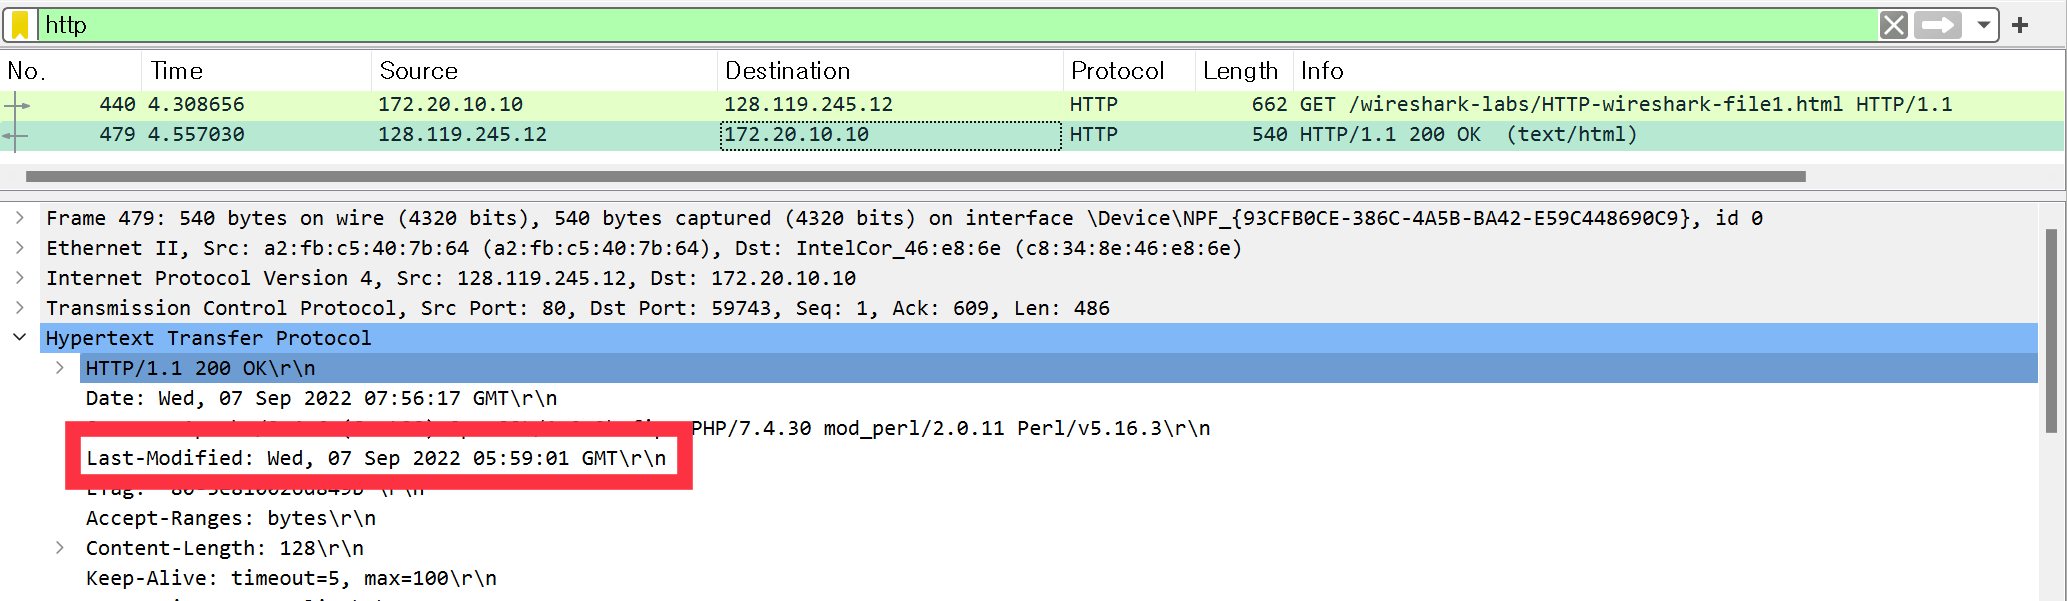
\includegraphics[width=.79\textwidth]{image/result_week01/Q2-5.png}
        		\caption{\footnotesize Problem 2-5's screenshot : Packet-HTTP/1.1 200 OK}
        		\vspace{-10pt}
            \end{figure}            
        \item How many bytes of content are being returned to your browser? \\[0.2mm]
            \soln 128 bytes
            \vspace{-2mm}  
            \begin{figure}[!h]\centering
        		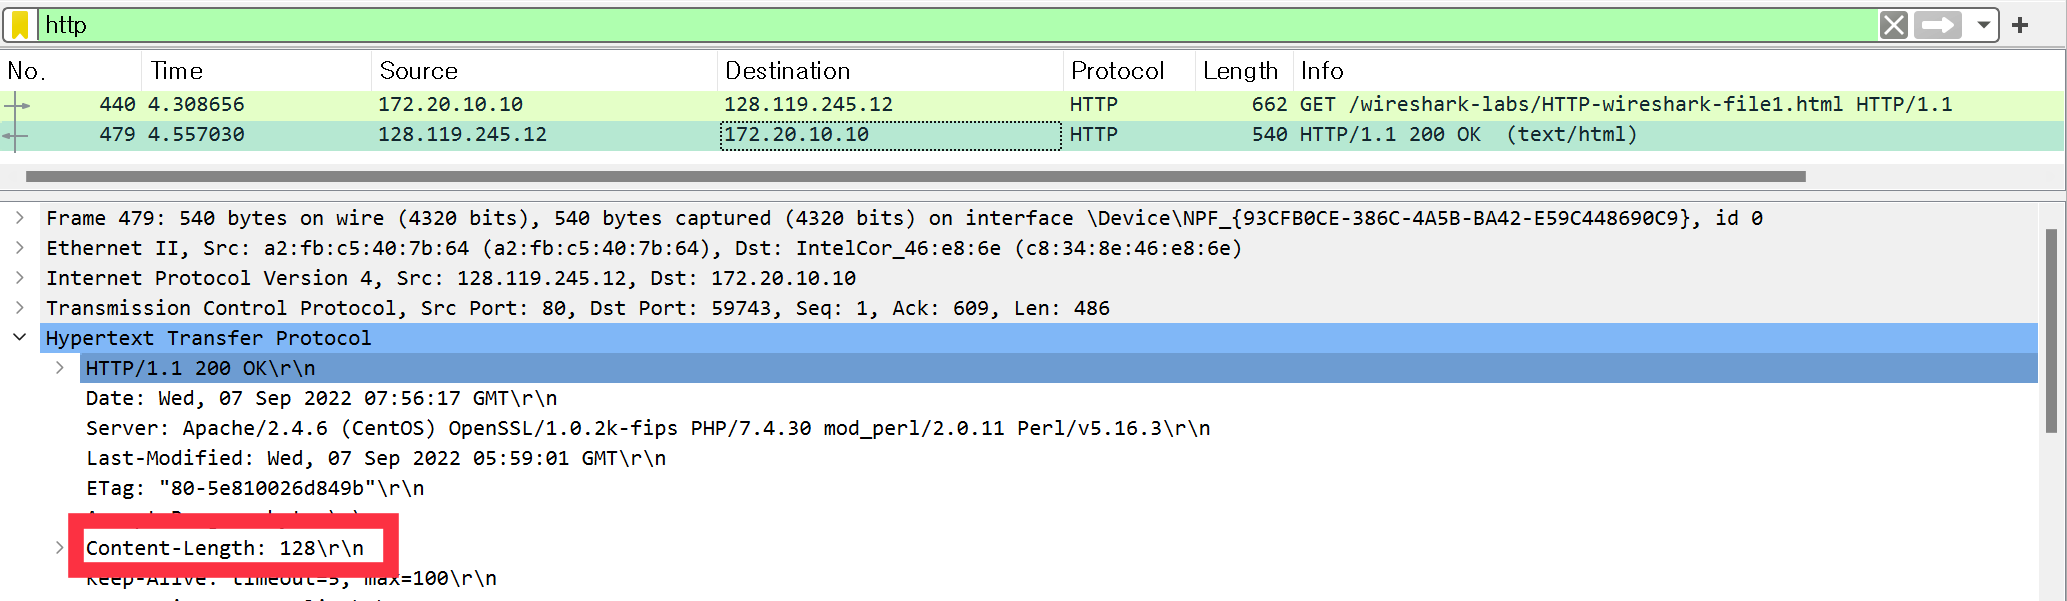
\includegraphics[width=.79\textwidth]{image/result_week01/Q2-6.png}
        		\caption{\footnotesize Problem 2-6's screenshot : Packet-HTTP/1.1 200 OK}
        		\vspace{-10pt}
            \end{figure}            
        \item By inspecting the raw data in the packet content window, 
        do you see any headers within the data that are not displayed in the packet-listing window?
        If so, name one.\\[0.2mm]
            \soln No, There are no headers in the HTTP Message below.
            
\newpage
    \end{enumerate}
\subsection{HTTP : The HTTP CONDITIONAL GET/response interaction}
    \subsubsection*{Problems}
    \begin{enumerate}[label=\bfseries Problem \arabic*:,leftmargin=*,labelindent=1em]\addtocounter{enumi}{7}
        \item Inspect the contents of the first HTTP GET request from your browser to the server.
        Do you see an “IF-MODIFIED-SINCE” line in the HTTP GET? \\[0.2mm]
            \soln There is no “IF-MODIFIED-SINCE” in the first GET packet.
            % \vspace{-2mm}  
            \begin{figure}[!h]\centering
        		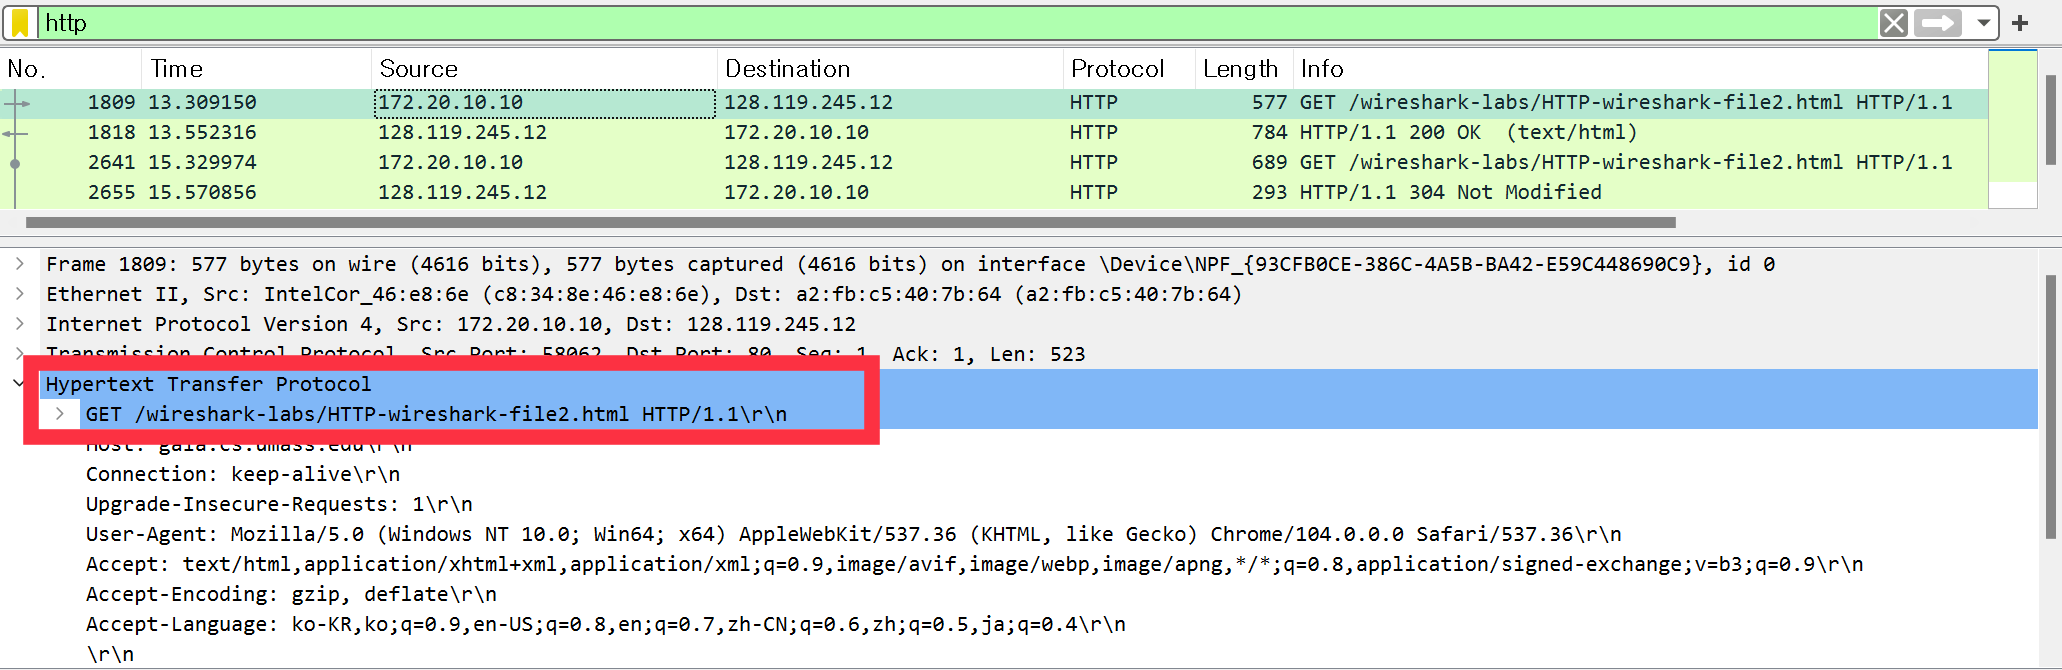
\includegraphics[width=.78\textwidth]{image/result_week01/Q2-8.png}
        		\caption{\footnotesize Problem 2-8's screenshot : Packet-GET / wireshark-file2.html HTTP/1.1}
        		\vspace{-10pt}
            \end{figure}    
        \item Inspect the contents of the server response. Did the server explicitly return 
        the contents of the file? How can you tell? \\[0.2mm]
            \soln Yes. The server explictly returned the contents of the html file.
            % \vspace{-2mm}  
            \begin{figure}[!h]\centering
        		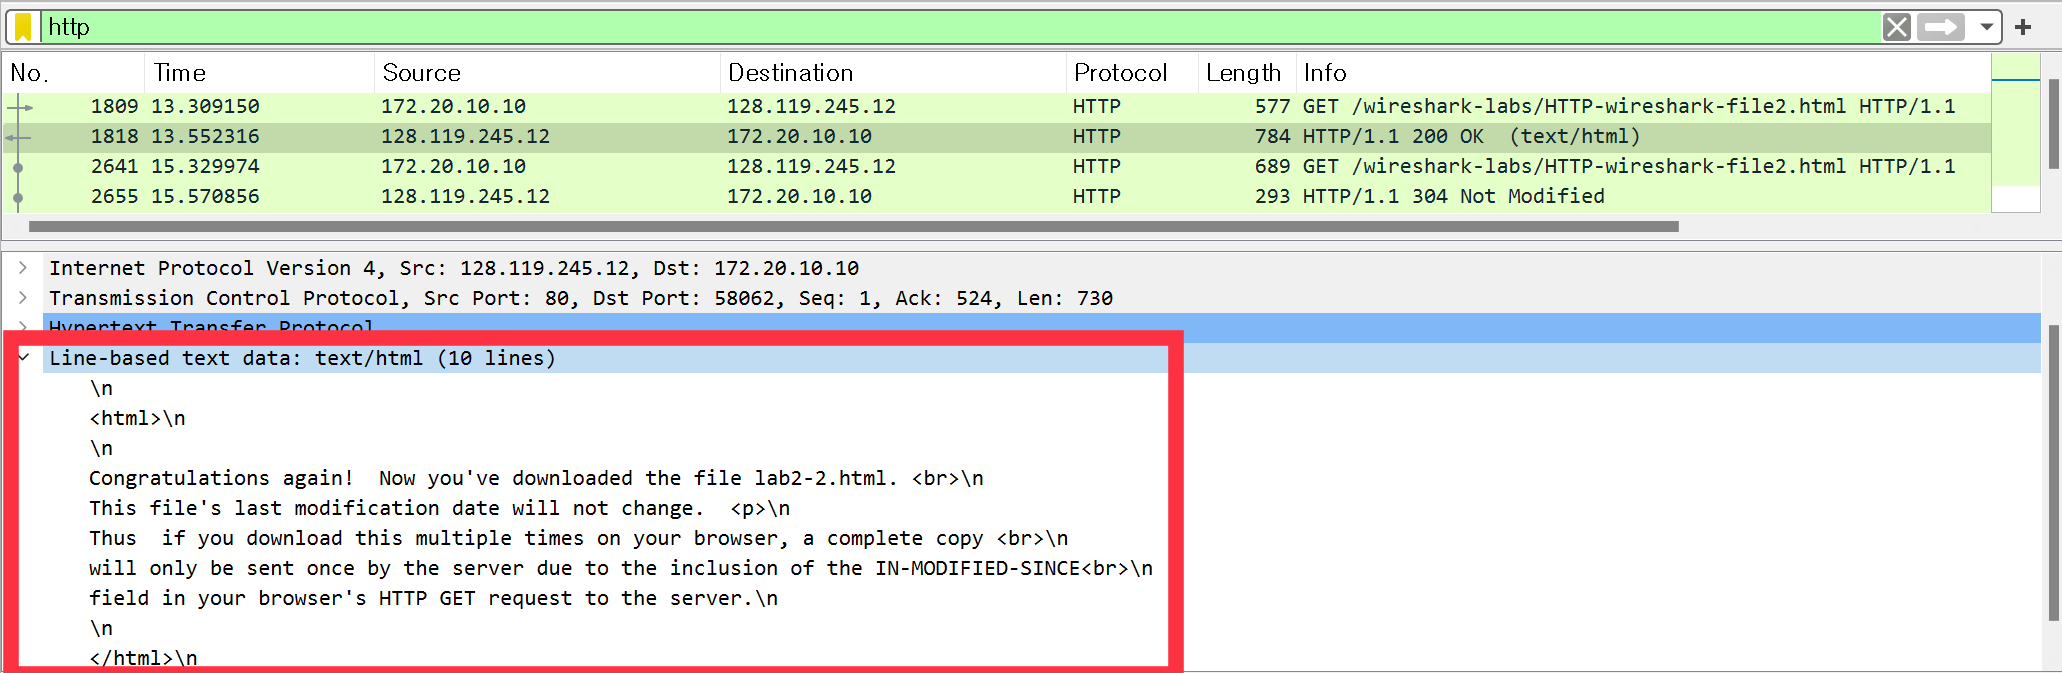
\includegraphics[width=.79\textwidth]{image/result_week01/Q2-9.png}
        		\caption{\footnotesize Problem 2-9's screenshot : Packet-HTTP/1.1 200 OK}
        		\vspace{-10pt}
            \end{figure}           
        \item Now inspect the contents of the second HTTP GET request from your browser to the server. Do you see an “IF-MODIFIED-SINCE:” line in the HTTP GET? If so, what information follows the “IF-MODIFIED-SINCE:” header?\\[0.2mm]
            \soln Yes. The information folloewed as 'wed, 07 sep 2022 05:59:01 GMT'
            % \vspace{-2mm}  
            \begin{figure}[!h]\centering
        		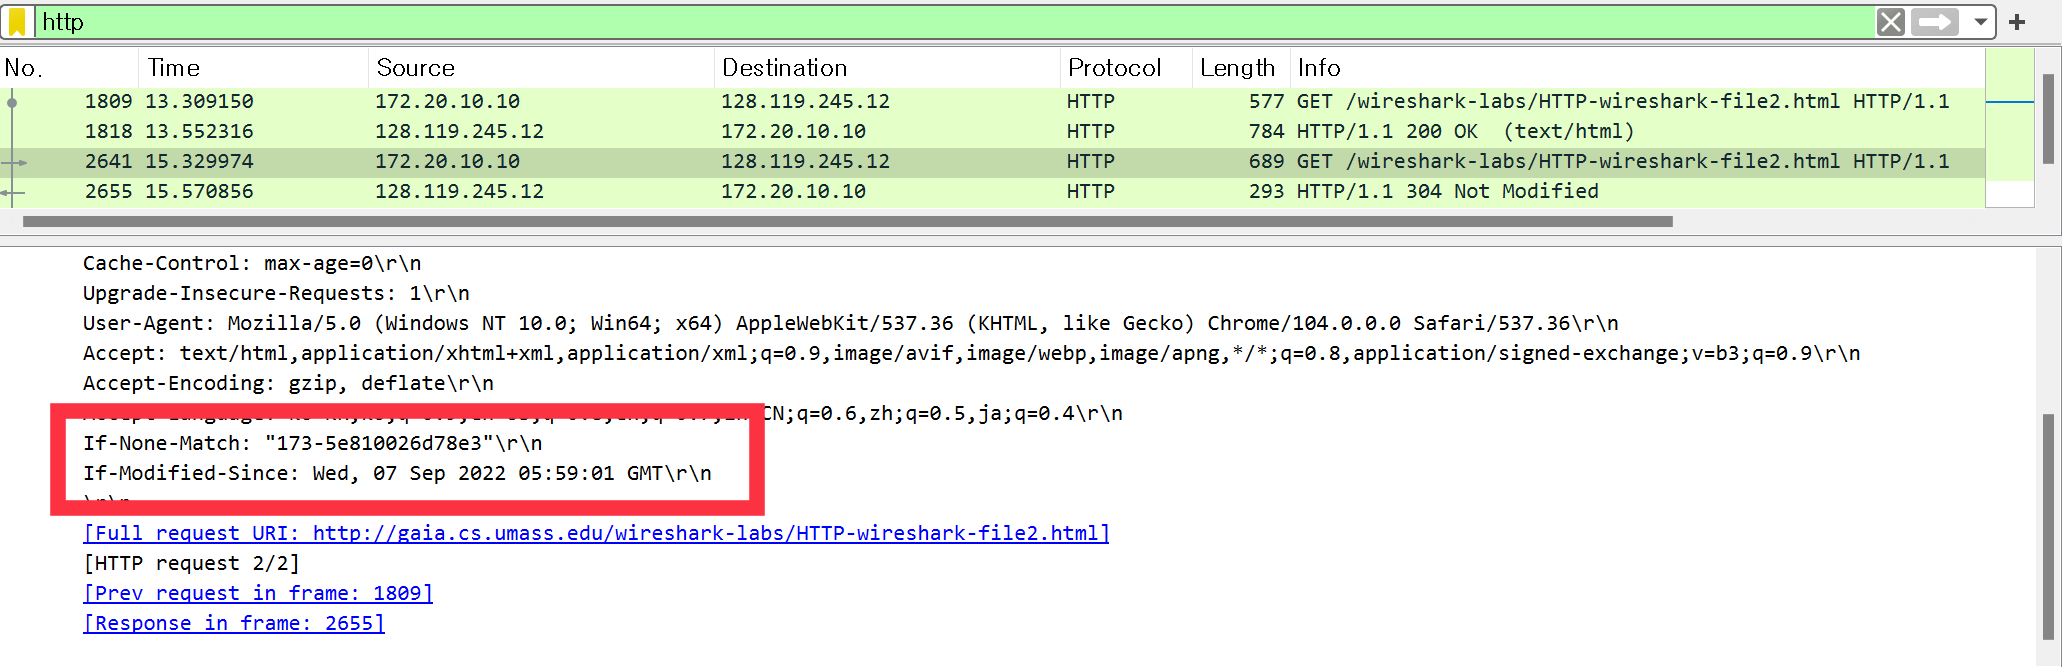
\includegraphics[width=.78\textwidth]{image/result_week01/Q2-a.png}
        		\caption{\footnotesize Problem 2-10's screenshot : Packet-GET / wireshark-file2.html HTTP/1.1}
        		\vspace{-10pt}
            \end{figure}           
        \item What is the HTTP status code and phrase returned from the server in response to this second HTTP GET? Did the server explicitly return the contents of the file? Explain.\\[0.2mm]
            \soln The status code and phrase returned from the server is ‘HTTP/1.1 Note Modified’.\\
            Since the browser loaded the file data from the browser’s cache\footnote{That, file hasnt’s been modified},
            the server not returned the file contents.
\newpage
            \vspace{-2mm}  
            \begin{figure}[!h]\centering
        		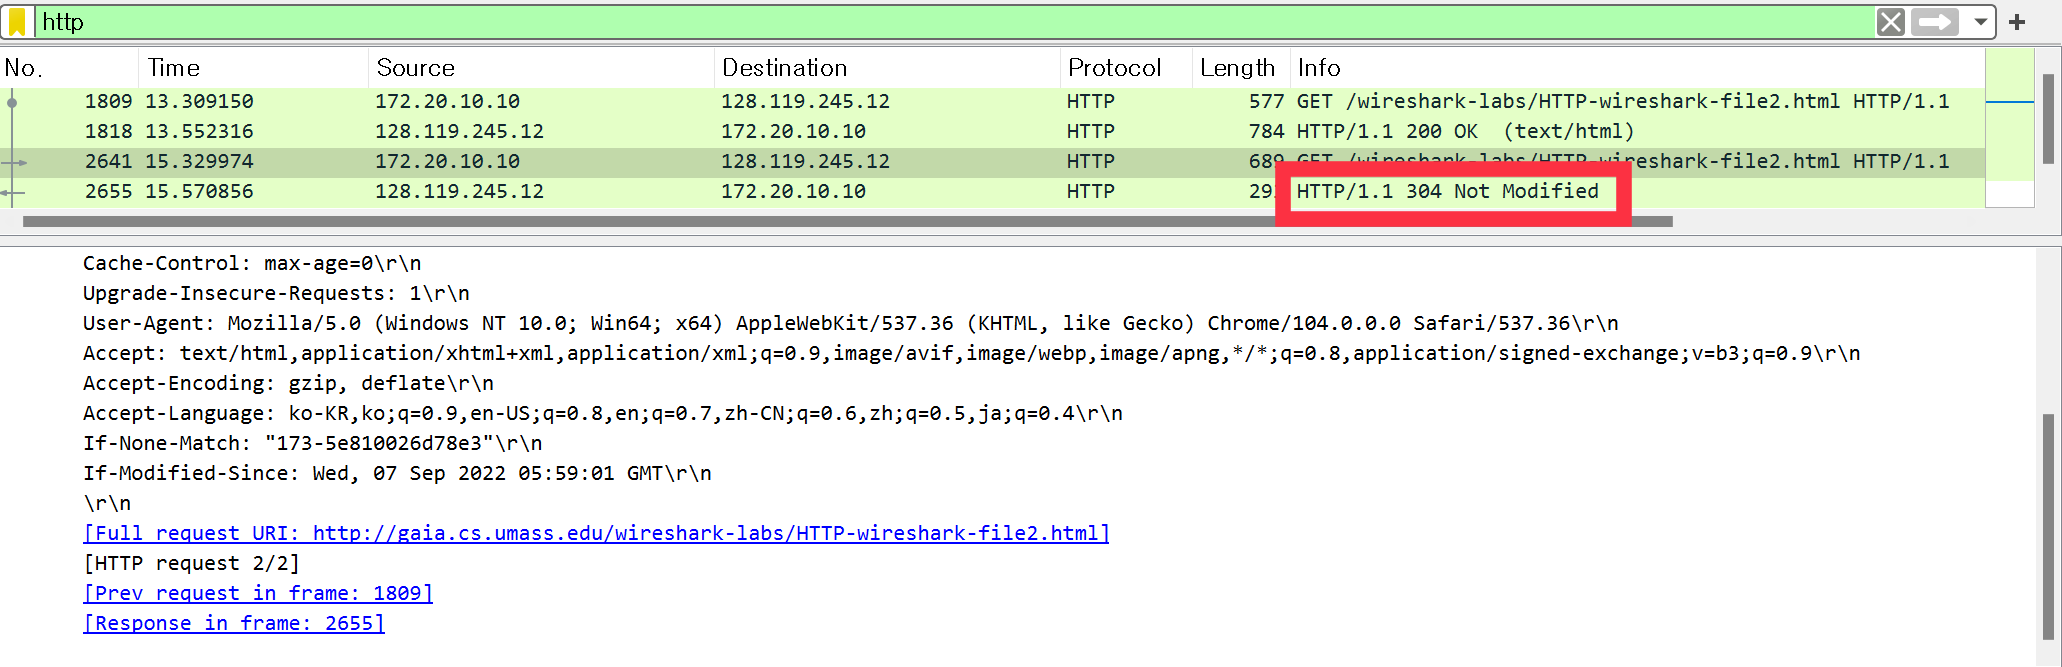
\includegraphics[width=.79\textwidth]{image/result_week01/Q2-b.png}
        		\caption{\footnotesize Problem 2-11's screenshot : Packet-HTTP/1.1 304 Not Modified}
        		\vspace{-10pt}
            \end{figure}            
    \end{enumerate}
\subsection{HTTP : Retrieving Long Documents}
    \subsubsection*{Problems}
    \begin{enumerate}[label=\bfseries Problem \arabic*:,leftmargin=*,labelindent=1em]\addtocounter{enumi}{11}
        \item How many HTTP GET request messages did your browser send? \\[0.2mm]
            \soln  1 times / Packet no.42
            \begin{figure}[!h]\centering
        		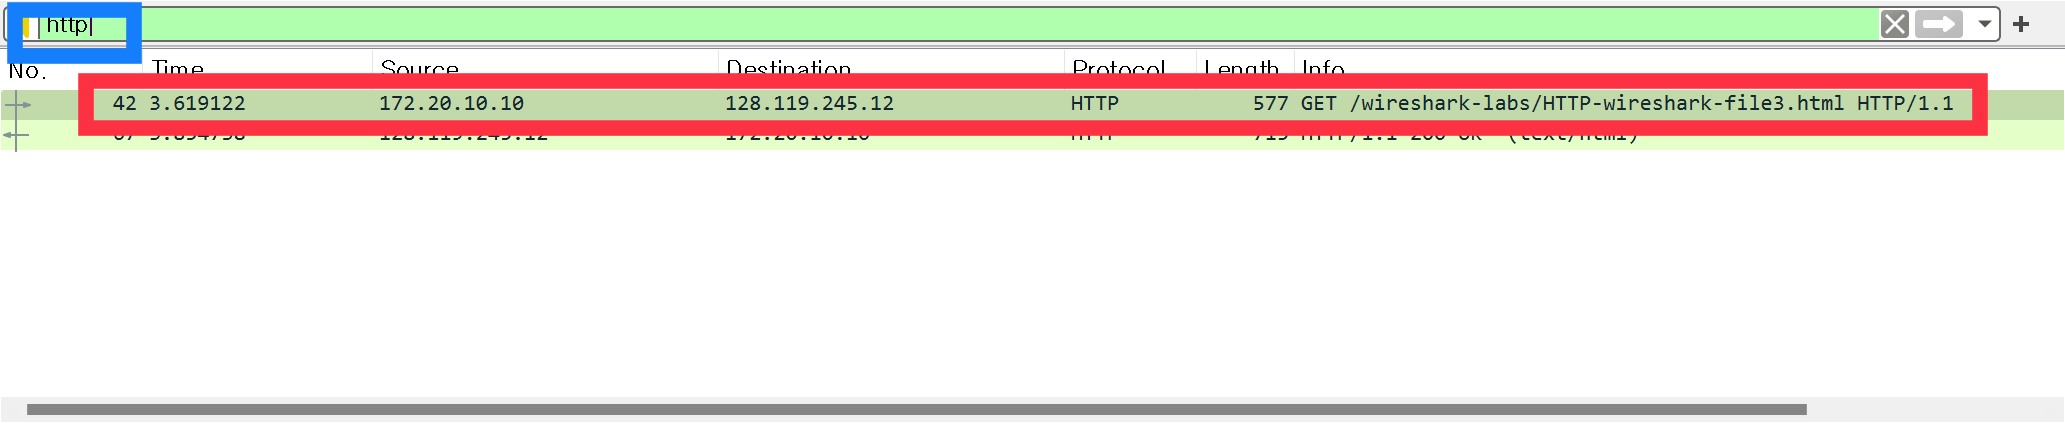
\includegraphics[width=.78\textwidth]{image/result_week01/Q2-c.png}
        		\caption{\footnotesize Problem 2-12's screenshot : Captured packet lists filterd by keyword 'http' getting file3}
        		\vspace{-10pt}
            \end{figure}   
        \item Which packet number in the trace contains the status code and phrase associated with the response to the HTTP GET request?\\[0.2mm]
            \soln  Packet no.67 
            \begin{figure}[!h]\centering
        		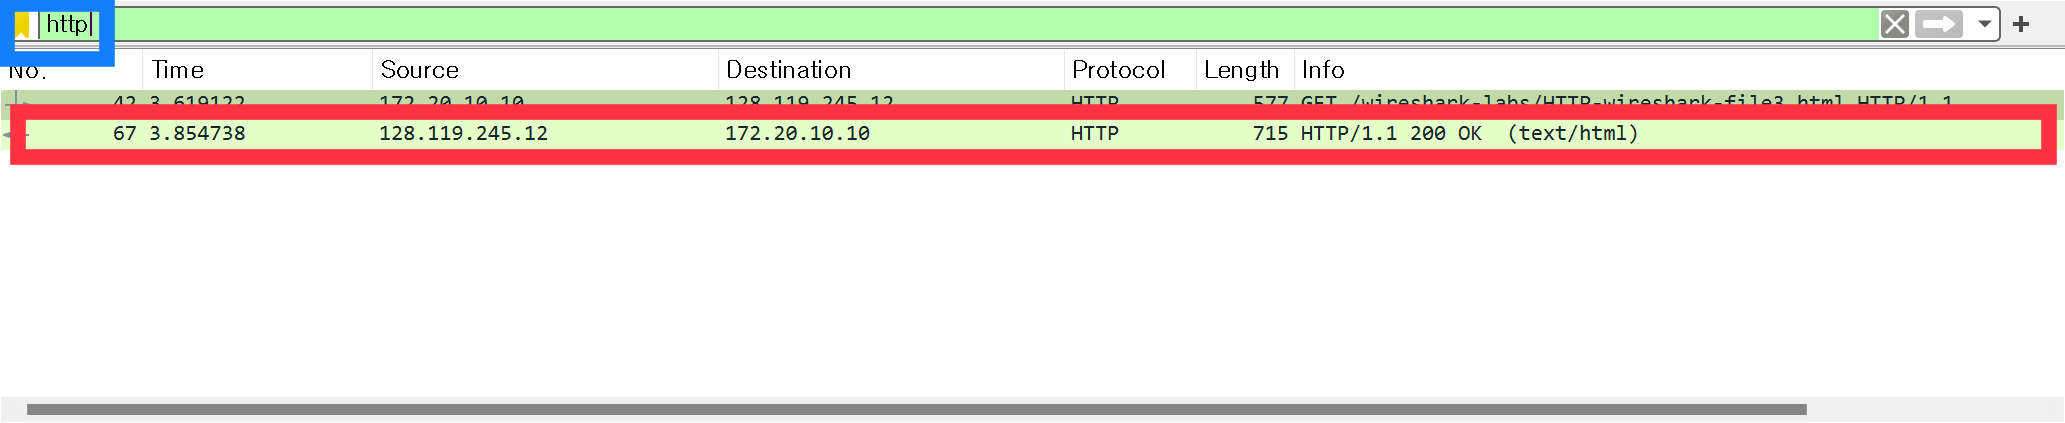
\includegraphics[width=.78\textwidth]{image/result_week01/Q2-d.png}
        		\caption{\footnotesize Problem 2-13's screenshot : Captured packet lists filterd by keyword 'http' getting file3}
        		\vspace{-10pt}
            \end{figure}            
        \item What is the status code and phrase in the response?\\[0.2mm]
            \soln Status code : 200 / Phrase : OK
            \begin{figure}[!h]\centering
        		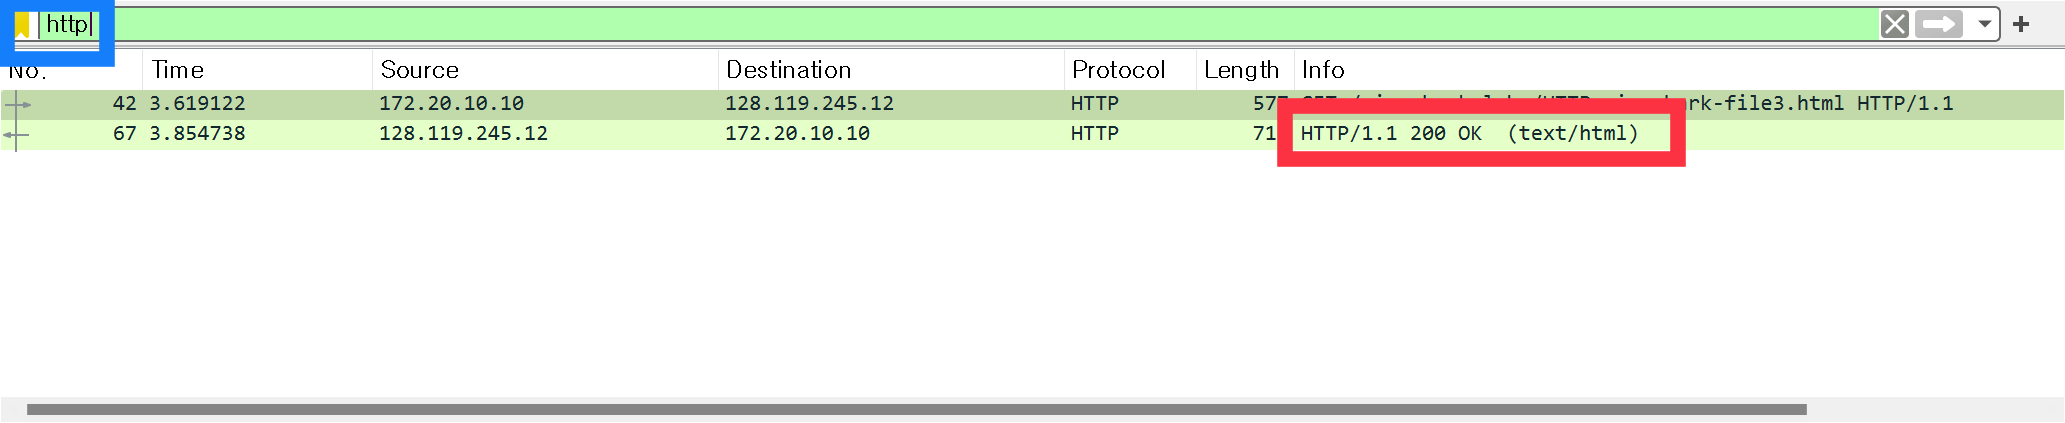
\includegraphics[width=.78\textwidth]{image/result_week01/Q2-e.png}
        		\caption{\footnotesize Problem 2-14's screenshot : Captured packet lists filterd by keyword 'http' getting file3}
        		\vspace{-10pt}
            \end{figure}   
        \item How many data-containing TCP segments were needed to carry
        the single HTTP response and the text of the Bill of Rights? \\[0.2mm]
            \soln \\
            Three packets. There are three data-containing TCP segments needed to transport the single HTTP response and the 
            text in the bill of Rights in wireshark-lab file3.
\newpage
            \begin{figure}[!h]\centering
        		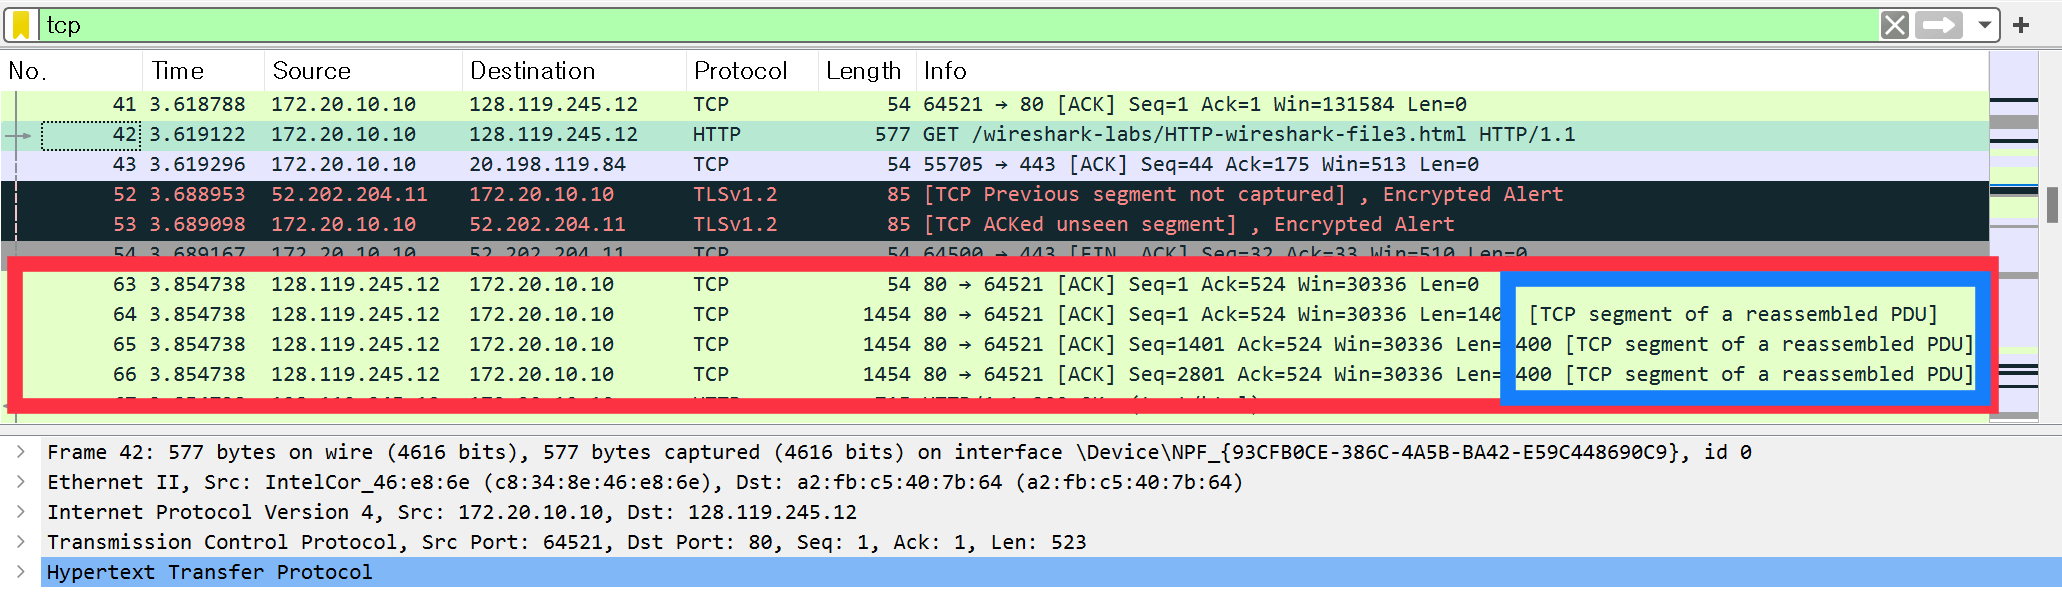
\includegraphics[width=.85\textwidth]{image/result_week01/Q2-f.png}
        		\caption{\footnotesize Problem 2-15's screenshot : Captured packet lists filterd by keyword 'TCP'}
        		\vspace{-10pt}
            \end{figure}  
    \end{enumerate}